\section{Evaluation}\label{sec:evaluation}
\subsection{Performance Model}
We build a performance model as follows: (We referred to GROUP 11)\\

Serial Performance \\
$S = N^3 * T$\\

Parallel Speedup \\
$ Speedup = S / ( Overhead + S / p ) $\\

where $N$ is the number of vertices $T$ is time to execute atomic operations,
$Overhead$ is the overhead time for parallelization such as communicating and
$p$ is the number of cores we can use.

The basic intuition behind this simple model is that as we can increase the
$N$, the number of vertices, we could achieve the higher speed up, and the
overhead becomes smaller relatively. 

%Justin%
\subsection{OpenMP Scaling}

\begin{figure}[H]
    \centering
    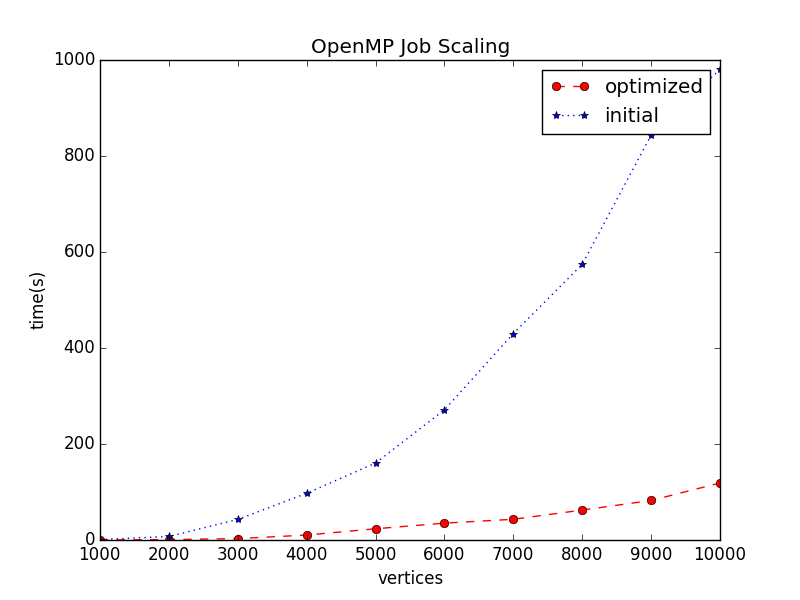
\includegraphics[width=0.8\textwidth]{figs/MPI_job_scaling.png}
    \caption{OpenMP Job Scaling with 1 Node - 24 Threads}
\end{figure}

The picture shows the scaling paradigm of the original code and optimized OpenMP code. From this picture, we can
see there is a factor of 10 improvement after our optimization. This picture also gives information about the
scaling of the calculation. Non-linear regression fit of this curve gives a result of $O(N^{3.22})$. \\

In theory, this algorithm should have a $O(N^{3})$ scaling with respect to one single iteration. The result
different from the idea case because for a smaller graph, it can be fit into cache.

\subsection{MPI Scaling}

\begin{figure}[H]
    \centering
    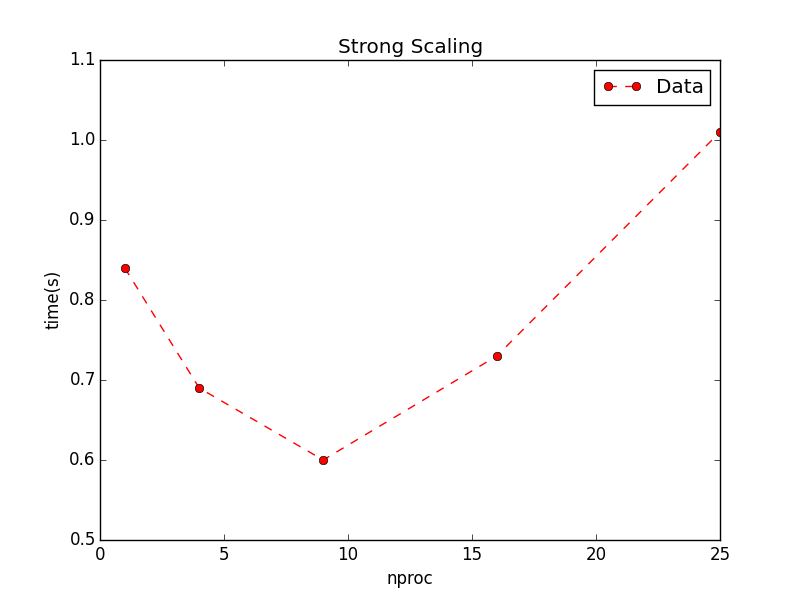
\includegraphics[width=0.6\textwidth]{figs/MPI_strong_scaling.png}
    \caption{MPI Strong Scaling Naive}
\end{figure}

This is our first implementation of MPI code, tested with 2000 by 2000 graph. This strong scaling diagram shows the communication
overhead is very big, and it's performance is no better than serial code at very large number of ranks. 

\subsection{Non-Blocking Communication}

Notice that we don't need the whole column and row of the matrix to begin the shortest path calculation, we just need the first
column block and first row block, then we can do the calculation. So we implemented a new version of MPI based on non-blocking
communication \textcolor{blue}{MPI\_Ibcast}. The procedure is as follows:
\begin{enumerate}
\item The rank owning the first column block or row block do a blocking board-cast.
\item The rank owning the second column block or row block do a non-blocking board-cast.
\item Wait for the first column block and row block.
\item Update the graph based on the first column block and row block.
\item The rank owning the third column block or row block do a non-blocking board-cast.
\item Wait for the second column block and row block.
\item Go to the 4th step.
\end{enumerate}

After the optimization, we can see improvement.
\begin{figure}[H]
    \centering
    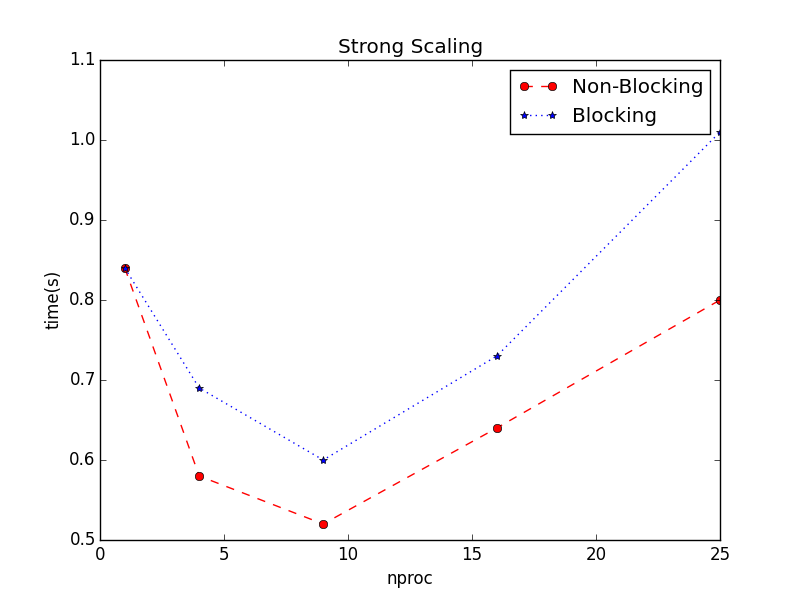
\includegraphics[width=0.6\textwidth]{figs/strong_scaling.png}
    \caption{MPI Strong Scaling Non-Blocking}
\end{figure}

\subsection{MPI Weak Scaling}
Since this algorithm is not linear scaling, it is hard to define weak scaling, because the problem size grows $O(N^{3})$.
The data tested is listed below:
\begin{equation*}
\begin{tabular}{c|ccccc}
      & 1      & 4 & 9 & 16 & 25       \\
\hline 
2000  & 0.84   &   &   &    &          \\
4000  & 5.74  &  2.79 &   &   &       \\
6000  & 13.30  &   &  16.40 &    &     \\
8000  & 23.59   &   &   &  68.91  &    \\
10000 & 33.18   &   &   &    &  162.419  \\
\end{tabular}
\end{equation*}

From this graph, we can calculate the speed up factor represented in the following graph.
\begin{figure}[H]
    \centering
    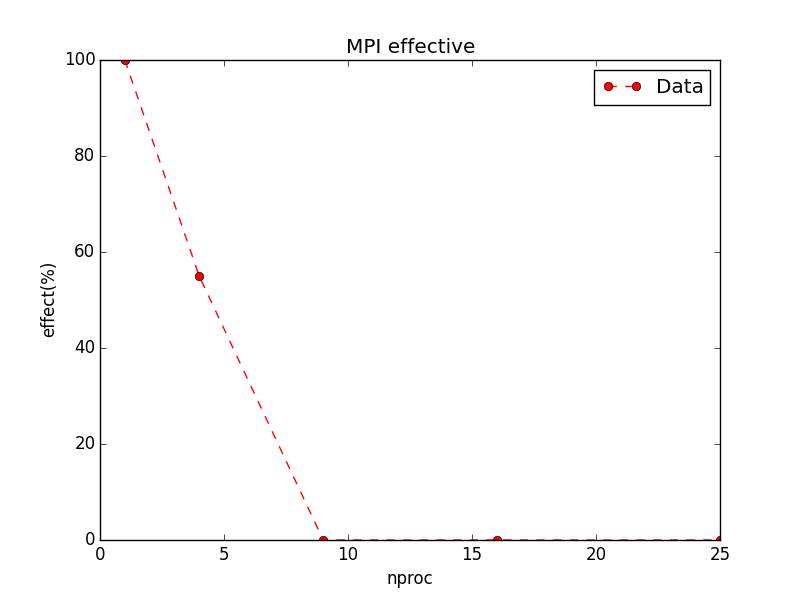
\includegraphics[width=0.45\textwidth]{figs/MPI_effective.png}
    \caption{MPI Effective}
\end{figure}

From the result above, MPI is not used effectively. We think one reason is that the calculation of
one single job is too small, because this algorithm uses additions to update the graph. So the
fraction of Communication vs Calculation will be really high. \\
